\documentclass[10pt]{article}
\usepackage[breaklinks=true]{hyperref}
\usepackage[margin=0.75in]{geometry}

\usepackage{textcomp}
\usepackage{color}
\usepackage{graphicx}
\definecolor{pblue}{rgb}{0.13,0.13,1}
\definecolor{pgreen}{rgb}{0,0.5,0}
\definecolor{pred}{rgb}{0.9,0,0}
\definecolor{pgrey}{rgb}{0.46,0.45,0.48}

\usepackage{listings}
\lstset{language=bash,
  showspaces=false,
  showtabs=false,
  breaklines=true,
  showstringspaces=false,
  tabsize=2,
  breakatwhitespace=true,
  commentstyle=\color{pgreen},
  keywordstyle=\color{pblue},
  stringstyle=\color{pred},
  numbers=left,
  stepnumber=1,
  basicstyle=\small\ttfamily,
  frame=single,
  moredelim=[il][\textcolor{pgrey}]{$$},
  moredelim=[is][\textcolor{pgrey}]{\%\%}{\%\%}
}

\title{\textbf{Week 09} \\
\LARGE Apache2 and Flask \\
\Large Making a Professional Webserver}
\author{
	Melvyn Ian Drag
}
\date{\today}


\begin{document}
\maketitle

\begin{abstract}
Last class we took a look at the toy `SimpleHTTPServer' in Python3. Tonight we'll use a real website backend - Flask - and we'll server content on a real server - Apache2. As before, we'll make \textbf{GET} and \textbf{POST} requests using the command line tool cURL.
\end{abstract}

\section{Meta Data}

Still, we'll try and make tonight as `stand-alone' as possible. If you missed last week, you ought to read the notes to catch up on what curl is and how to use it.

\section{What's a Webserver?}
The term is overloaded. A server is a computer, connected to a network, that other computers can access. There may be more ways to define it, but that's what I think of. But for your midterm I had you install some postgresql server stuff. In that case I was referring to the database server software. And tonight I'm going to refer to Apache2 as a 'webserver' - it's actually software that runs \textit{on} a webserver, which is the machine. It's just that the terms are overloaded.

\section{What's Flask?}
Flask is what is called a \textbf{Library}. It's some code that you can use in a language to solve a particular problem. For example, if you know Java you've probably used the \textit{java.util} library for things like \textit{ArrayList}s. In Python last week we used a library calle \textit{SimpleHTTPServer} to serve up some webpages for us on the address \textit{localhost:8000}.

\section{What's a REST API}
Too many buzzwords out there. REST is an acronym. You can read about it more if you want. For the rest of the lecture just understand that you usually pass JSON data back and forth over a REST API. We'll talk about JSON later.

\subsection{Job interview prep}
\noindent\textit{\textbf{Interviewer:} I see you know a bit about Linux webserver maintenance. Do you know what a REST API is?}

\noindent \textbf{You: } Honestly, not too much because I'm not a webdeveloper. But I do know that REST APIs are very popular now, and they typically involve the exchange of JSON data. JSON data is when the data is structured like a Python dicitonary, or a Java Hashmap  - its a bunch of key-value pairs in curly braces.

If you can give the above answer, you'll know enough for now.

\section{What we'll do today}
Today we'll bring a real website online. Last week we made a trivial website with Python's SimpleHTTPServer, but today we're going to use a real, professional-grade server ( Apache2 ) and a real backend web framework ( Flask ). There are other servers like NGINX and there are other backend webframeworks like Django, Play, Spring, Ruby on Rails, etc., I've just chosen this pair because it's the easiest to code of the few things I know. Spring on NGINX would be considerably harder to configure.

\begin{figure}[h]
  \centering
    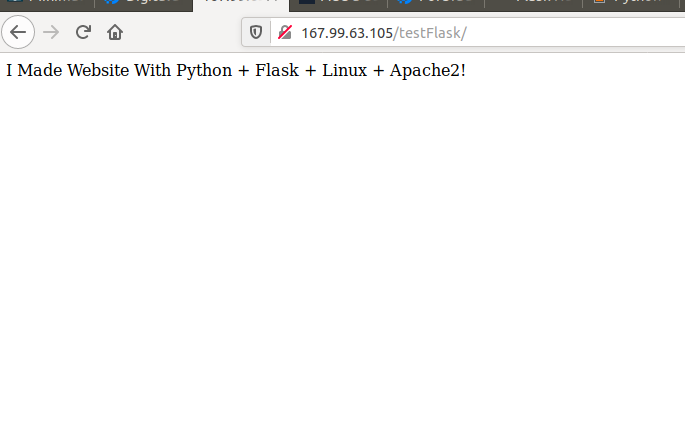
\includegraphics[width=0.8\textwidth]{Exercise1Success.png}
  \caption{A website running on my server at IP address http://167.99.63.105/testFlask/}
\end{figure}



\section{Setting up server}
Get a debian 10 server

\begin{lstlisting}
root@machine$ apt update
root@machine$ apt install apache2
root@machine$ apt-get install libapache2-mod-wsgi-py3 python3-dev python3-pip
root@machine$ pip3 install flask flask-restful
root@machine$ apt install curl
root@machine$ service apache2 status
# should report that apache2 is running
root@machine$ curl localhost
# lots of data
root@machine$ curl localhost > curlResponse.html
# dump the data to a file so it's easier to look through
root@machine$ less curlResponse.html # look through, verify you have the default apache page. That means the server is running.
root@machine$ curl ipinfo.io/io # get your server ip address
\end{lstlisting}

Open a browser on a laptop or computer. Go to the server ip address, make sure the server is running. You should see the same default apache page you saw with curl localhost. But now you are looking at it through a browser on a different machine ( you ran curl on the webserver itself ).

\begin{figure}[h]
  \centering
    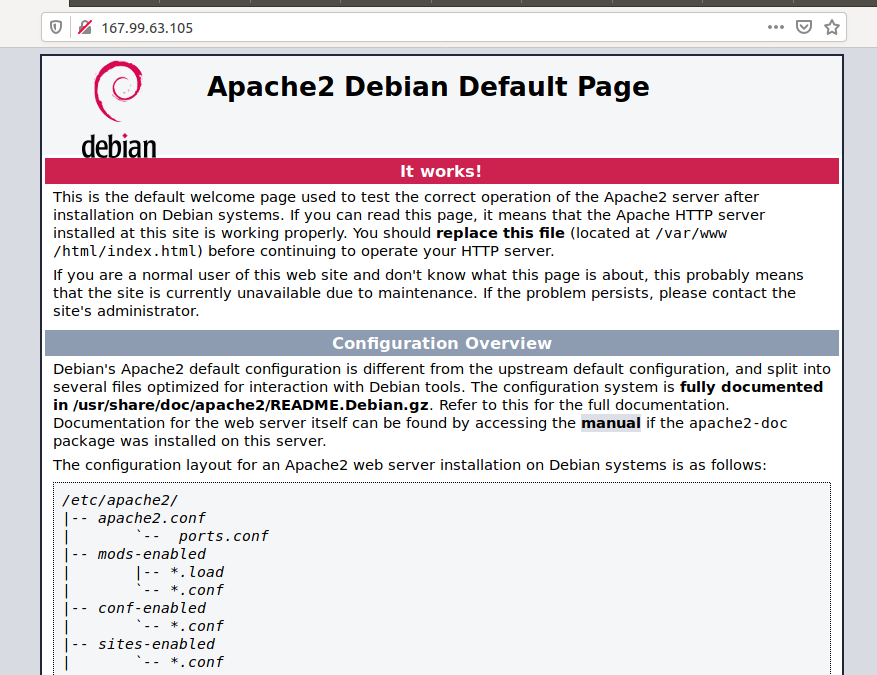
\includegraphics[width=0.8\textwidth]{defaultApache.png}
  \caption{default webpage provided by a fresh Apache2 install}
\end{figure}

So we've installed all the software we need! That was easy. Now we can build a little website and then connect the website code to the apache server we just installed and activated.

\section{Creating a Flask application}
The first thing we need to do is create a non root user for managing this stuff. We'll give the user sudo permission for the few root things we need to do to bring the website online. I've created user `webdeveloper'. You should do the same so you can copy and paste the code I've provided. If you create a different username, you'll need to make the minor modifications to make everyting match up.

\begin{lstlisting}
root@machine$ adduser webdeveloper
root@machine$ usermod -a -G sudo webdeveloper
root@machine$ sudo su - webdeveloper
root@machine$ mkdir /home/webdeveloper/ExampleFlask
\end{lstlisting}

Inside the ExampleFlask directory, put the files described below. Note that these files are available in the Example1/ExampleFlask directory in the class Git repo.

\subsection{\_\_init\_\_.py}
This is an empty file

\subsection{my\_flask\_app.py}
\lstinputlisting{Example1/ExampleFlask/my_flask_app.py}

\subsection{my\_flask\_app.wsgi}
\lstinputlisting{Example1/ExampleFlask/my_flask_app.wsgi}


\section{Connect Flask to Apache2}
Now we need to wire up our Flask application to the Apache webserver software. You will need to know your machine's ip address. I showed you a website you can curl that will tell you your ipaddress

\begin{lstlisting}
user@machine$ curl ipinfo.io/ip
# returns your external ip address
\end{lstlisting}

Then you need to create this file, and put the proper ip address. Note that you'll need to run vim with sudo as this is a privileged file.

\subsection{/etc/apache2/sites-available/ExampleFlask.conf}

\lstinputlisting{Example1/ExampleFlask.conf}

\subsection{Turn on and Test the Website}
Run these commands as the user `webdeveloper'
\begin{lstlisting}
webdeveloper@machine$ sudo a2ensite ExampleFlask
webdeveloper@machine$ sudo a2enmod wsgi
webdeveloper@machine$ sudo service apache2 restart
\end{lstlisting}

Then, open a browser on your laptop or the NJCU PC in front of you and go to 

\begin{center}
\textit{my.ip.addr.ess/testFlask}
\end{center}

You should see a message saying you've made your first website with Linux, flask, apache and python. You can share the link to show off your website to your friends and family! You could now also go to godaddy or namecheap, buy a domain name, and wire that up to your server so people can go to website.com instead of a scary looking ip address.

\section{Additional Considerations for Example 1}
So we have a simple flask app running on apache now. As you've probably seen by now, Linux servers are very particular about groups and permissions. I'm not sure about all of the ins and outs of the permissions for Flask and Apache. I'm showing the permisisons and groups I've set up on my machine. If you do something else I'm not sure it will work, and I don't know why it owuld be broken. We could experiment with permissions if you have something else.


I'm also not sure about all the details of the ExampleFlask.conf file. There are many options to it. I've always set mine up by scouring the internet for information and banging in what ever details I found. I hope to one day understand this file in depth, but for now all I know is how to make it work.

\begin{figure}[h]
  \centering
    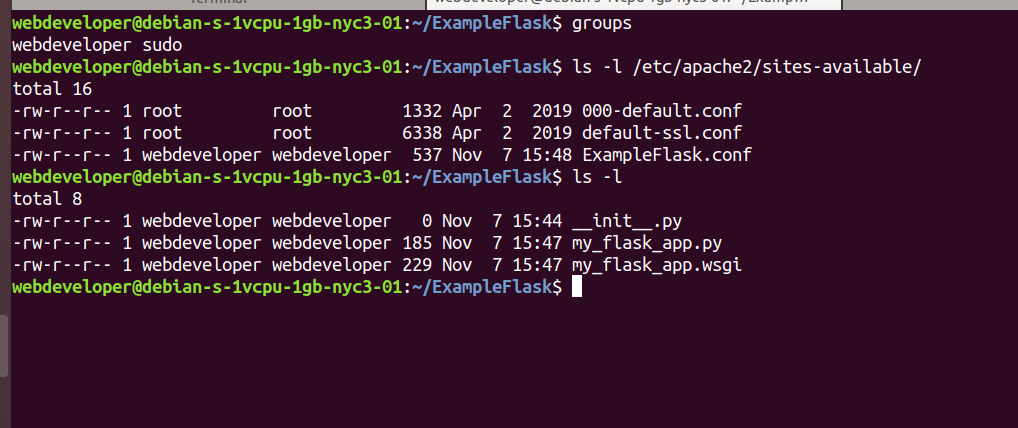
\includegraphics[width=0.8\textwidth]{groupsAndPermissions.png}
  \caption{My permissions and groups on a successful install}
\end{figure}

{\LARGE Wait for class to all be caught up and have their servers running}

\section{About the code for Example 1}
This isn't a Python class as we said, but I'll just mention a few things about the Python code so you get some sense of how it's working. You will see the line

\begin{lstlisting}[language=Python]
@app.route("/")
def hello():
	return "some string here"
\end{lstlisting}
 
This says that when we GET the location "/" in our domain name, the webserver will respond with the return value.

We have to go to "ipaddress/testFlask" to see this data because in our config file we have the line

\begin{lstlisting}
...
WSGIScriptAlias /testFlask /home/webdeveloper/ExampleFlask/my_flask_app.wsgi
...
\end{lstlisting}

and this registers the base end point for our website as /testFlask. If there's time we can change this. Right now apache is serving the default apache website on /, so we had to put our website at a different location on our server. Well need to delete some config files and change this config file so that we can see our website when we go to "/" instead of having to go to "/testFlask".

The contents of the .wsgi file is boilerplate stuff that won't matter to you unless you want to become a serious python developer. Also, the purpose of the .wsgi file is interesting, but probably won't matter to you. Python applications can't run natively on webservers. So, about 20 years ago, some developers go together and wrote some middleware that allowds Python applications to communicate with webserver software like Apache2. The details are complicated - you can read about it if you're curious. 

\url{https://en.wikipedia.org/wiki/Web_Server_Gateway_Interface}

I think php can talk right to the webserver, but I'm not sure. I've never written a line of php in my life. All I know is that PYhton needs a thing called wsgi ( which we installed at the beginning of this lecture with libapache-mod-wsgi-py3 ). You'll note that there are different version for python3 and python2.

\section{Example2: Adding Endpoints and Serving HTML}
To do this
\begin{enumerate}
\item Change the ExampleFlask.conf file to the one below.
\item Create the /home/webdeveloper/Example2 directory add the files from the class repo
\item Restart apache2
\end{enumerate}

\subsection{New /etc/apache2/sites-available/ExampleFlask.conf}
Note that this file now serves two webpages! You can host multiple websites on one webserver.
\lstinputlisting{Example2/ExampleFlask.conf}

\subsection{my\_flask\_app.py}
\lstinputlisting{Example2/ExampleFlask2/my_flask_app.py}

\subsection{my\_flask\_app.wsgi}
\lstinputlisting{Example2/ExampleFlask2/my_flask_app.wsgi}

\subsection{\_\_init\_\_.py}
Blank as before. To be honest I haven't given it thought if this is required or not. Just put the file. If you know python you can remove it and then meditate on why it works / doesn't work if you remove this file.

\subsection{ Results }
Here are some images showing my new site in action. The /testFlask endpoint still works, but now so do /somewhereElse and /somewhereElse/returnsHTML.

\begin{figure}[h]
  \centering
    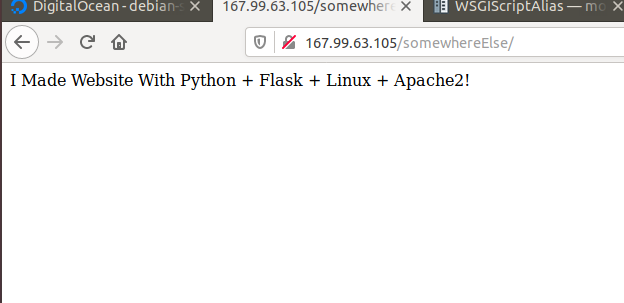
\includegraphics[width=0.8\textwidth]{somewhereElse.png}
  \caption{somewhereElse now works}
\end{figure}

\begin{figure}[h]
  \centering
    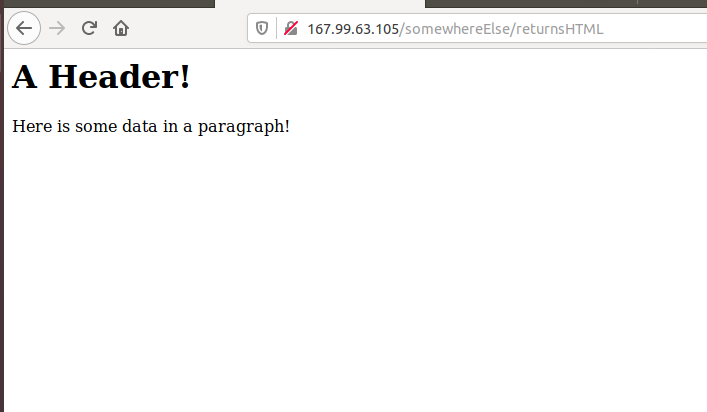
\includegraphics[width=0.8\textwidth]{somewhereElse_returnsHTML.png}
  \caption{We can now return HTML from our Flask website too!}
\end{figure}

{\LARGE Wait for class to all be caught up and have their servers running again}

\section{Example3: A Rest API}
{\LARGE Only do this section if the class is caught up and it's before 9 PM}

So far we've returned plain text and text formatted as HTML from our website. A popular thing to do now is to pass around JSON data. JSON is used all over. I showed it to you last week just to wet your feet, but you'll see it everywhere. You'll use it for web programming, internally in Python code, passing data between applications running on a laptop, for exchanging data files with scientists - everywhere. I avoided JSON for a while because I thought it was just a stupid buzz word that the nerds used to show off, but it truly is an ubiquitous data format. Now you've seen it. You'll see it again, mark my words. 

So we'll just see how to return json from a Flask application.

Just as we did in example 2, set up your server with Example3 now. Get the Example3 code from github, copy the new ExampleFlask.conf file to the proper location in /etc, create the /home/webdeveloper/Example3 directory, and put the proper code in it. 

\subsection{The Flask Application: my\_flask\_app.py}
You can skim the code to see what it does. It has some code for handling the GET and POST requests. A GET request will echo back to you the entire contents of the TODOS data it's maintaining. A POST request will add to the TODOS data set. You can verify after POSTing that your data was added by sending a GET request.

\lstinputlisting{Example3/ExampleFlask3/my_flask_app.py}

\subsection{Accessing Our REST API}
Then you can get JSON data in the browser as shown below:

\begin{figure}[h]
  \centering
    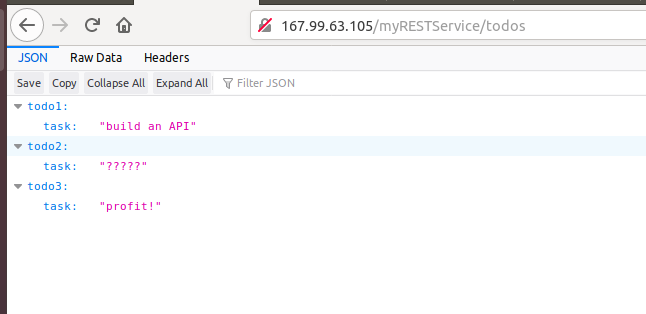
\includegraphics[width=0.8\textwidth]{restInBrowser.png}
  \caption{See some json in the browser!}
\end{figure}

Then, on your laptop, make a GET request with cURL


\begin{figure}[h]
  \centering
    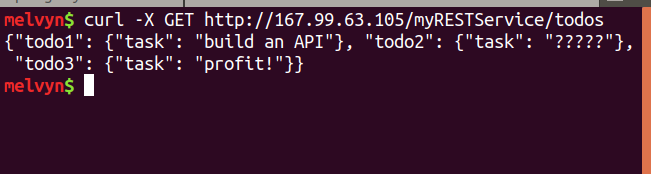
\includegraphics[width=0.8\textwidth]{curlYourAPI.png}
  \caption{Make a GET request with cURL!}
\end{figure}

And, you should also be able to make the following POST request:

\lstinputlisting{curlExample.sh}

And then look, after POSTing data, when you GET data you will see the data that you POSTed!

\begin{figure}[h]
  \centering
    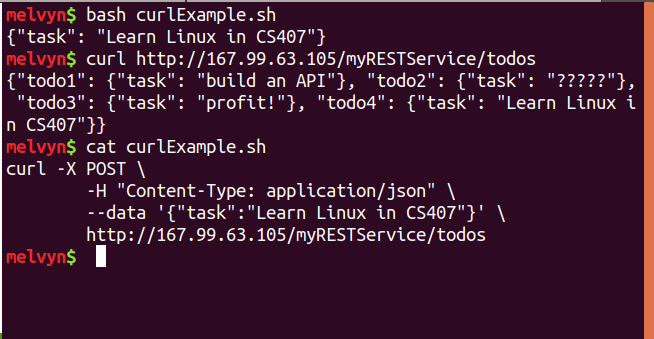
\includegraphics[width=0.8\textwidth]{addedToTODOList.png}
  \caption{POST data to your website with cURL!}
\end{figure}

\pagebreak

\section{Flask and Bigger Websites}
Typically your website code will return HTML. I've only shown you how to return HTML strings in example 2, but typically you create HTML templates and populate the template with data. Too complicated to explain, there is no time. Google 'Flask and HTML templates' if you want to know more.

NOTE if class ends early, we can do this together, but I suspect we'll be plenty busy tonight.

\section{Databases}
For your exam you set up a postgres server with some data in it. I've just shown you how to set up a Flask web application on an Apache server. And you have a good knowledge now about some linux server maintenance things. 

In the TODOList REST application we stored all of our data in a dictionary - in the real world this is not how you do it. Can you guess what you do for real websites? You use a DATABASE! You are now poised to go pick up a book on Flask and learn how to wire a database and a website backend together!

Of course we won't do that in this class, but now you have the prerequisite information to go and follow a tutorial on building websites with Flask.

\section{sed}
sed is one of the more popular command line tools. So far we know grep, vim, cat, mv, ls, etc.. sed is another one of the "big ones".

sed stands for ``stream editor" and is a simple little programming language ( or tool, depending how you want to view it ) that is used for processing text files line by line.

\subsection{What to do with sed \#1}
Sed can be used to replace all occurences of a string in a file.
See sedExamples/01.

\begin{lstlisting}
user@machine$ cat oldFile
user@machine$ sed 's/hello//' oldFile
# will replace first occurences of 'hello' with nothing\
# note that a line with two occurences of 'hello' will only have the first occurence replaced
user@machine$ cat oldFile
# the file is not changed. sed did not overwrite the original file
user@machine$ sed 's/hello/HELLO/' oldFile
# see first occurences of hello were replaced with HELLO
\end{lstlisting}

these changes were done in place. If you want to create a new file you can do it like this

\begin{lstlisting}
user@machine$ sed 's/hello/HELLO' <oldFile >newFile
user@machine$ sed 's/hello/HELLO' oldFile >newFile
user@machine$ sed 's/hello/HELLO' 0<oldFile >newFile
# all of the above are equivalent
\end{lstlisting}

or you can change the input file in place

\begin{lstlisting}
sed -i  's/HELLO/hewwo/' newFile
\end{lstlisting}

the -i means `in place'.

\subsection{What to do with sed \#2}
We saw sed can do search and replace first occurence per line. It can also replace all occurrences in a file.

\begin{lstlisting}
user@machine$ sed 's/hello/HELLO/g' oldFile
#note all occurences of hello now say HELLO
\end{lstlisting}

by adding the g after the search/replace pattern you can replace all occurences.

\subsection{What to do with sed \#3}
Sed can do regular expressions. If you want to capitalize any 'h' at the start of a line, you can do this:

\begin{lstlisting}
user@machine$ sed 's/\(^[h]\)//' oldFile
ello world
ello world world
world hello hello world
\end{lstlisting}

\subsection{What to do with sed \#4}
You can also extract patterns. This is a weird thing that you can't always do with things like search/replace in microsoft word/excel/whatever other tools you are familiar with.

the same command as before remembers and stores the search pattern in a variable called \textbackslash1. You can do the same thing with \textbackslash2, \textbackslash3, etc for subsequent search patterns. \textbf{The search patterns are the regexs enclosed in \textbackslash( and \textbackslash)}. In the example above, my regex was looking for a line that starts with h. If you scroll down a bit youll see a regex for a line that starts with an ASCII letter.

\begin{lstlisting}
sed 's/\(^[h]\)/\1\1\1/' oldFile
hhhello world
hhhello world world
world hello hello world
\end{lstlisting}

You may not be mentally prepared to appreciate what I've just shown you? Maybe one day you'll be trying to do a complicated search and replace task and then you'll remember sed!

Check out this interesting example too!

\begin{lstlisting}
user@machine$ sed 's/\(^[a-zA-Z]\)/\1\1\1/' oldFile
hhhello world
hhhello world world
wwworld hello hello world
\end{lstlisting}

If I want to wrap the first letter of every line with smileys, for example, I can do this:

\begin{lstlisting}
user@machine$ # emojis!
user@machine$ sed 's/\(^[a-zA-Z]\)/\xF0\x9F\x98\x82\1\xF0\x9F\x98\x82/' oldFile
# look what comes out! Depending on your laptop, the output will be different from the output I have as can be seen in the figure below
\end{lstlisting}


\begin{figure}[h]
  \centering
    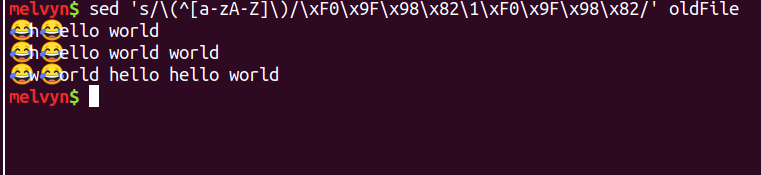
\includegraphics[width=0.8\textwidth]{mayOrMayNotWorkForYou.png}
  \caption{How the heck did he do that? If you already know, I'm very impressed}
\end{figure}

But this may or may not work on your computer, we'll talk about this in depth if there is time this semester.

\subsection{It's not Halloween, I don't want to scare you}
So far today I've showed you what to type to turn on an Apache webserver and we copy and pasted some Python Flask code. Then I showed you a whole new programming language called `sed'. Well, sed isn't quite a language. It is and it isn't, depends on what you want to define as a programming language. You've seen it can be used for search and replace. And you've seen that it can use regexes.

\begin{center}
{\LARGE Questoin for class: What is REGEX short for?What are some tools you already know that use regular expressions?}
\end{center}


Here is a site that will teach you a ton about sed:
http://www.grymoire.com/Unix/Sed.html

in fact, you will need to read this website for your homework. Theres so much to know, I've only shown you the tip of the iceberg. You can go now and learn as much as you care to, I think you understand enough to hit the ground running. There is also a super famous book out there about sed \& a related language called awk:

You could spend 20-30 bucks here for it:
https://www.amazon.com/sed-awk-Dale-Dougherty/dp/1565922255

Or you can take it for free from this class repo! Inthe reading materials directory you will find the book sedandawk.pdf

There is alot to know to be a power Linux user and you already know alot, that's great, good for you!

\section{Recap of what you know}
\begin{enumerate}
\item A bit about the Bash programming language
\item grep \& regular expressions
\item What a user is on Linux
\item What a group is on Linux
\item What is git?
\item You're comfortable using a command line interface now
\item There are a few different languages on the command line - we've used bash and dash
\item What permissions are and how to modify them
\item What is a root user
\item What is a process
\item What is a job
\item How to send signals to processes ( kill, CTRL+C, CTRL+Z )
\item How to make code ignore or block signals
\item How to install software on Linux
\item A cool trick for using setuid / setgid to make a non-root user do some root stuff
\item basics of relational dbs and how to configure one on Linux
\item What is cron
\item curl
\item some vocabulary like API, REST, regex, SQL, DB
\item A bit about python programming
\item What is a website backend? Set up a website backend with Apache2 + Flask
\item What is sed?
\end{enumerate}

\section{Coming Up In This Class}

We have a few more important things to cover
\begin{enumerate}
\item set up a git server
\item add a gitlab front end to the git server
\item Linux and Text encodings
\item xxd, everyone's favorite binary packet analyzer
\item The AWK programming language
\item The hows and whys of formatting harddrives, usb sticks, solid state drives, etc.
\item Encryption with gpg + pgp. How it relates to ssh and other pub/priv key schemes.
\end{enumerate}

\section{References}
This lecture was based on what I read  on these websites:

\url{https://www.codementor.io/abhishake/minimal-apache-configuration-for-deploying-a-flask-app-ubuntu-18-04-phu50a7ft}



There were some bugs in the tutorials above that I sorted out to make sure our lecture had a good flow.
\end{document}
